\documentclass[aspectratio=169, table]{beamer}
\usepackage[utf8]{inputenc}
\usepackage[T1]{fontenc}
\usepackage{graphicx}
\usepackage{fontspec}
\usepackage{xcolor}
\usepackage{tcolorbox}
\usepackage{listings} % Add the listings package
\usepackage{hyperref} % Add the hyperref package

\lstdefinelanguage{JavaScript}{
    keywords={function, var, let, const, if, else, for, while, return, true, false},
    keywordstyle=\color{blue}\bfseries,
    ndkeywords={class, export, boolean, throw, implements, import, this},
    ndkeywordstyle=\color{orange}\bfseries,
    identifierstyle=\color{black},
    sensitive=false,
    comment=[l]{//},
    morecomment=[s]{/*}{*/},
    commentstyle=\color{gray}\ttfamily,
    stringstyle=\color{green}\ttfamily,
}

\lstset{
    breaklines=true,
    language=JavaScript,
    % ... (other style settings)
}

\lstdefinelanguage{PHP}{
    keywords={class, function, echo, if, else, foreach, for, while, return},
    keywordstyle=\color{blue}\bfseries,
    ndkeywords={public, private, protected, static},
    ndkeywordstyle=\color{purple}\bfseries,
    identifierstyle=\color{black},
    sensitive=false,
    comment=[l]{//},
    morecomment=[s]{/*}{*/},
    commentstyle=\color{gray}\ttfamily,
    stringstyle=\color{green}\ttfamily,
}

\lstset{
    breaklines=true,
    language=PHP,
    % ... (other style settings)
}

\setsansfont[
  ItalicFont=fonts/TitilliumWeb-Italic.ttf,
  BoldFont=fonts/TitilliumWeb-Bold.ttf,
  BoldItalicFont=fonts/TitilliumWeb-BoldItalic.ttf,
]{TitilliumWeb-Regular.ttf}

\subtitle{IF120203-Web Programming}
\title{\Huge {\textbf{13: \\Finishing \& Web Socket}}}
\date[Serial]{\scriptsize {PRU/SPMI/FR-BM-18/0222}}
\author[Pradita]{\small {\textbf{PRADITA UNIVERSITY}}}

\usetheme{Pradita}

\begin{document}
\begin{frame}
    \titlepage
\end{frame}

\begin{frame}{Goals - Finishing \& Web Socket}
    \vskip1cm
    \begin{itemize}
        \item \textbf{Understanding Project Completion:} Crucial steps and best practices involved in finalizing a web projects.
        \item \textbf{Implementing Web Sockets:} Introduce the concept of Web Sockets and their role in real-time communication between a client and server, demonstrating their usage and benefits in web applications.
        \item \textbf{Integration of Web Sockets:} Showcase practical examples or case studies of integrating Web Sockets into web applications, highlighting their advantages over traditional HTTP requests.
        \item \textbf{Performance Optimization:} Discuss strategies to optimize web applications utilizing Web Sockets, focusing on minimizing latency and maximizing efficiency.
        \item \textbf{Application Use Cases:} Illustrate real-world scenarios where Web Sockets can significantly improve functionality, such as chat applications, collaborative tools, gaming, or live data updates.
    \end{itemize}
\end{frame}


\begin{frame}{Create converter-api.blade.php at views}
    \vskip1cm
    \begin{center}
        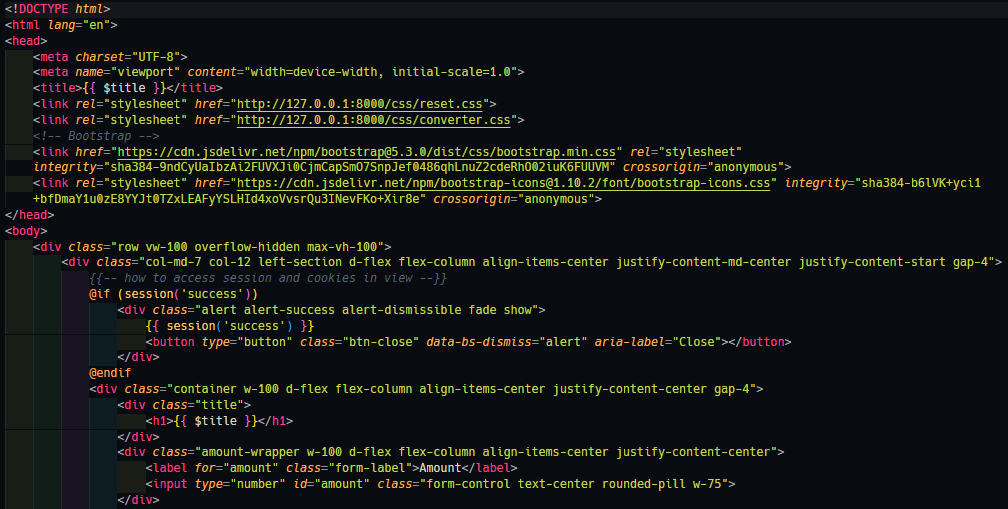
\includegraphics[width=0.8\textwidth]{classFiles/pertemuan-13-converter-api-part-1.png}
    \end{center}
\end{frame}

\begin{frame}{Create converter-api.blade.php at views}
    \vskip1cm
    \begin{center}
        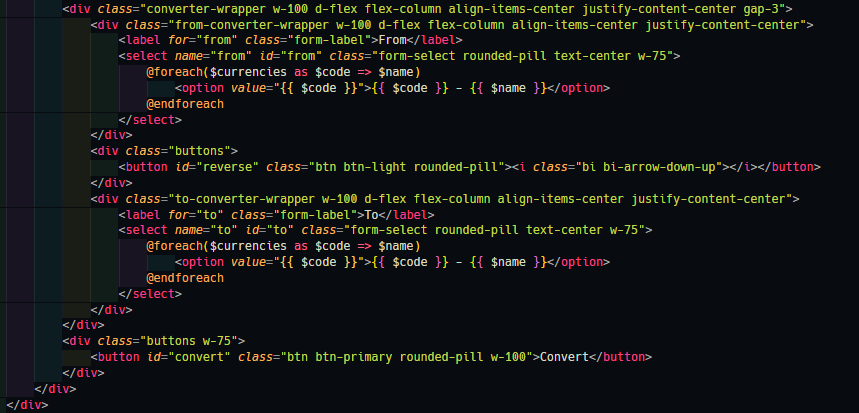
\includegraphics[width=0.8\textwidth]{classFiles/pertemuan-13-converter-api-part-2.png}
    \end{center}
\end{frame}

\begin{frame}{Create converter-api.blade.php at views}
    \vskip1cm
    \begin{center}
        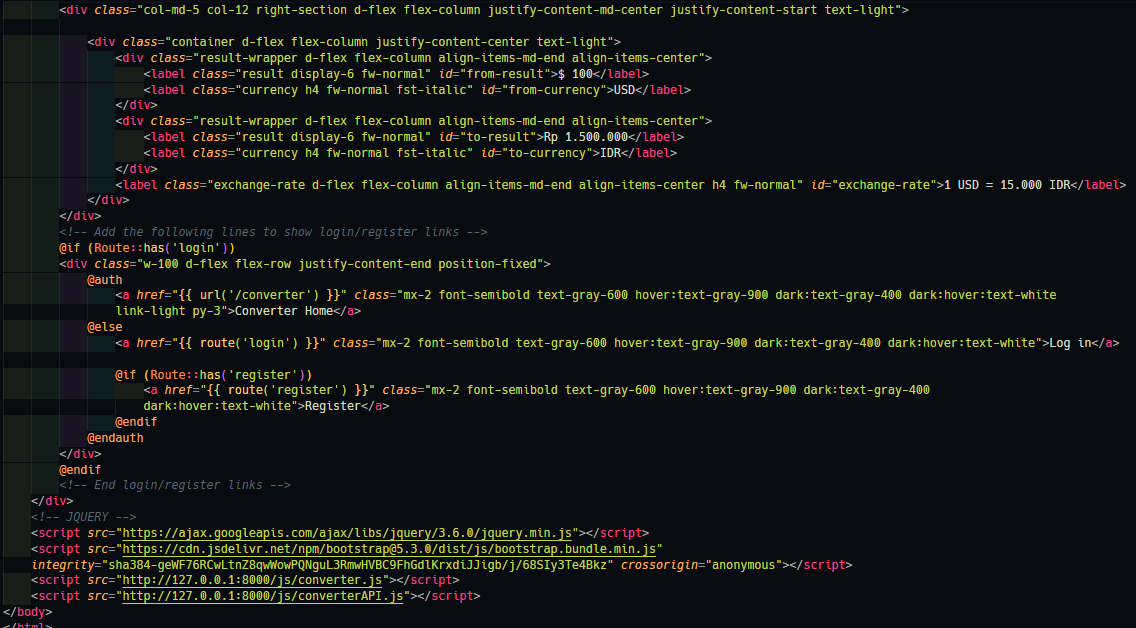
\includegraphics[width=0.8\textwidth]{classFiles/pertemuan-13-converter-api-part-3.png}
    \end{center}
\end{frame}

\begin{frame}{converter-database at views}
 \vskip1cm
 \begin{center}
  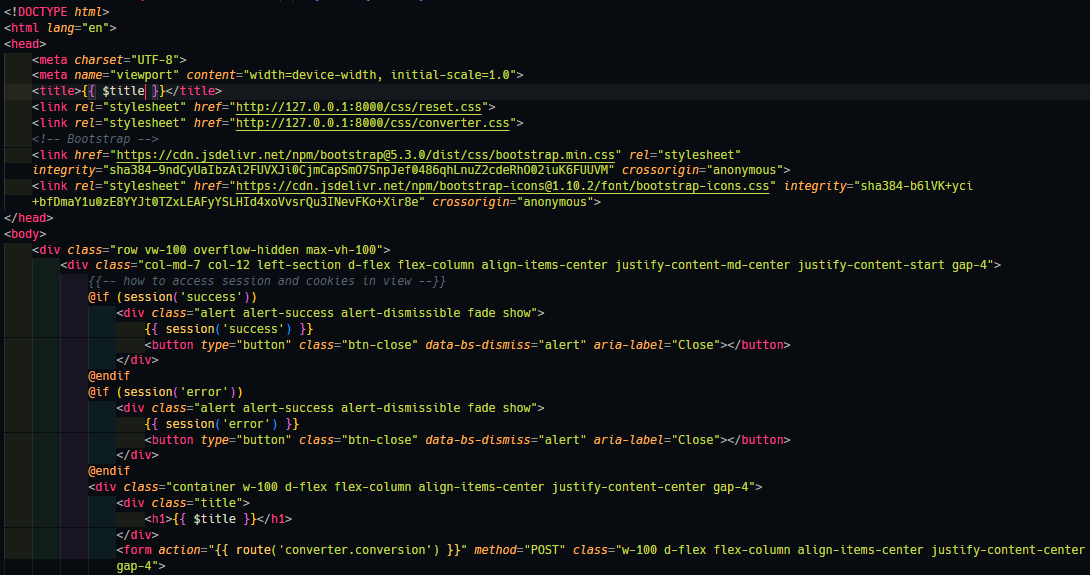
\includegraphics[width=0.8\textwidth]{classFiles/pertemuan-13-converter-database-part-1.png}
 \end{center}
\end{frame}

\begin{frame}{converter-database at views}
 \vskip1cm
 \begin{center}
  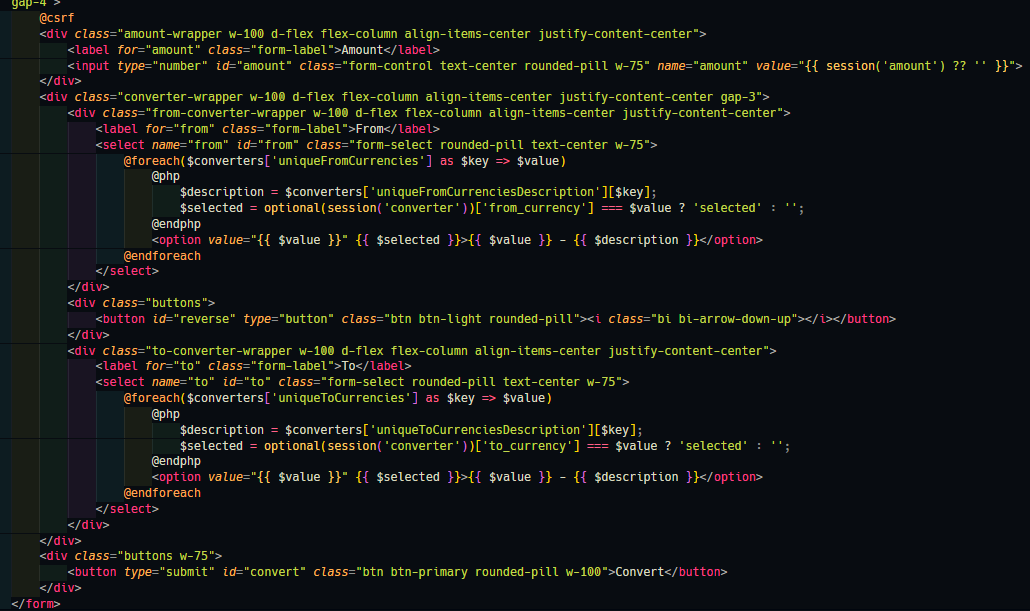
\includegraphics[width=0.8\textwidth]{classFiles/pertemuan-13-converter-database-part-2.png}
 \end{center}
\end{frame}

\begin{frame}{converter-database at views}
 \vskip1cm
 \begin{center}
  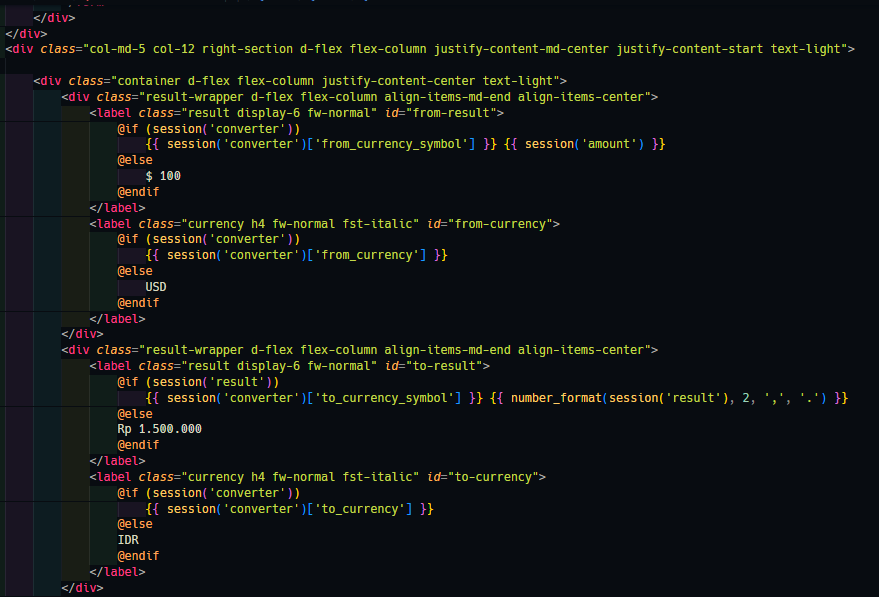
\includegraphics[width=0.8\textwidth]{classFiles/pertemuan-13-converter-database-part-3.png}
 \end{center}
\end{frame}

\begin{frame}{converter-database at views}
 \vskip1cm
 \begin{center}
  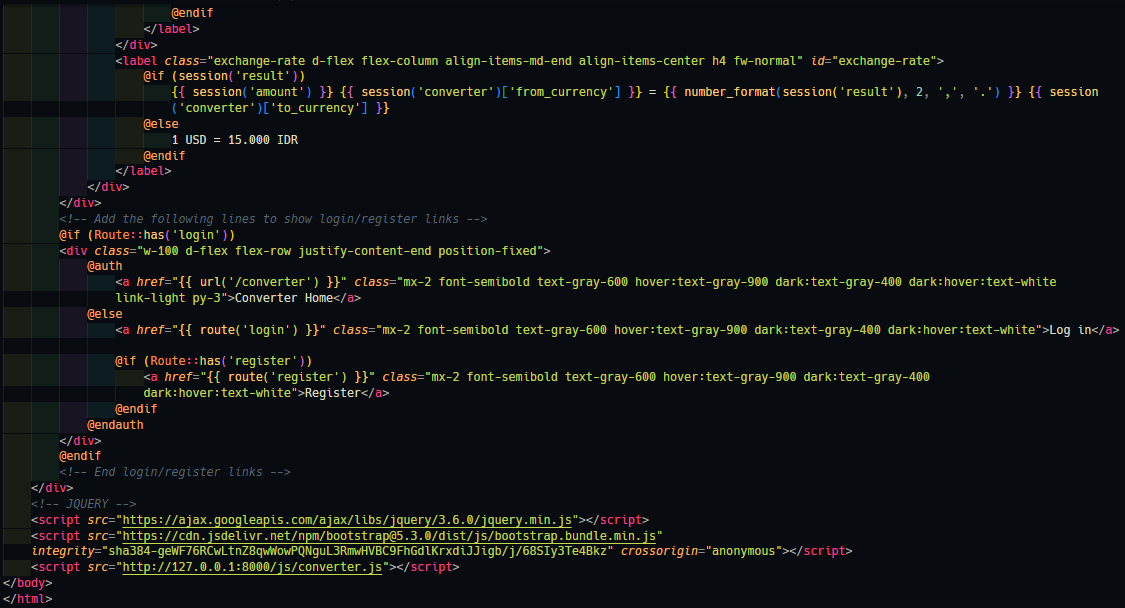
\includegraphics[width=0.8\textwidth]{classFiles/pertemuan-13-converter-database-part-4.png}
 \end{center}
\end{frame}

\begin{frame}{add api function at controller}
    \vskip1cm
    \begin{center}
        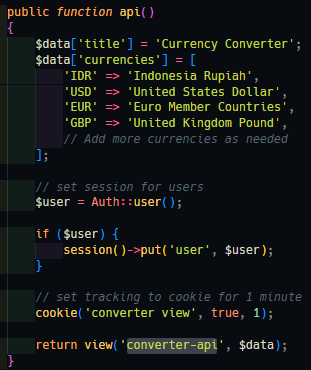
\includegraphics[width=0.4\textwidth]{classFiles/pertemuan-13-converter-controller-part-1.png}
       
        
        Add api function at ConverterController inside Controllers folder
    \end{center}
    \vfill % Pushes content to the bottom of the frame
\end{frame}

\begin{frame}{add auth middleware at controller}
    \vskip1cm
    \begin{center}
        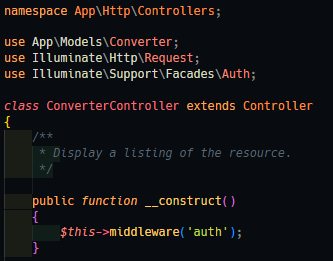
\includegraphics[width=0.4\textwidth]{classFiles/pertemuan-13-converter-controller-part-2.png}
       
        
        Add auth middleware at ConverterController inside Controllers folder
    \end{center}
    \vfill % Pushes content to the bottom of the frame
\end{frame}

\begin{frame}{add conversion function at controller}
    \vskip1cm
    \begin{center}
        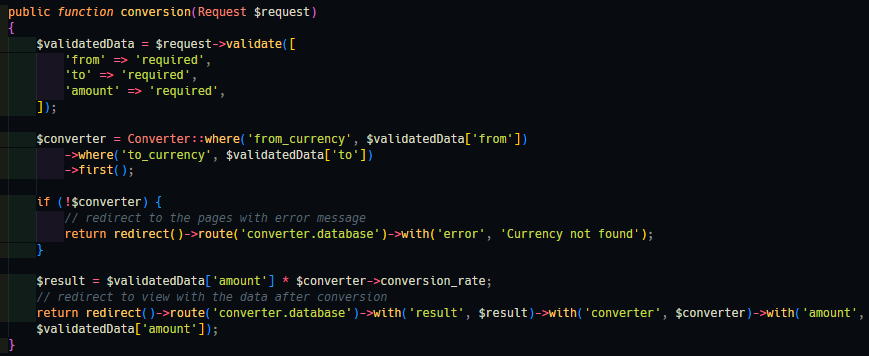
\includegraphics[width=0.6\textwidth]{classFiles/pertemuan-13-converter-controller-part-3.png}
       
        
        Add conversion function at ConverterController inside Controllers folder
    \end{center}
    \vfill % Pushes content to the bottom of the frame
\end{frame}

\begin{frame}{Add Routes in web.php routes}
    \vskip1cm
    \begin{center}
        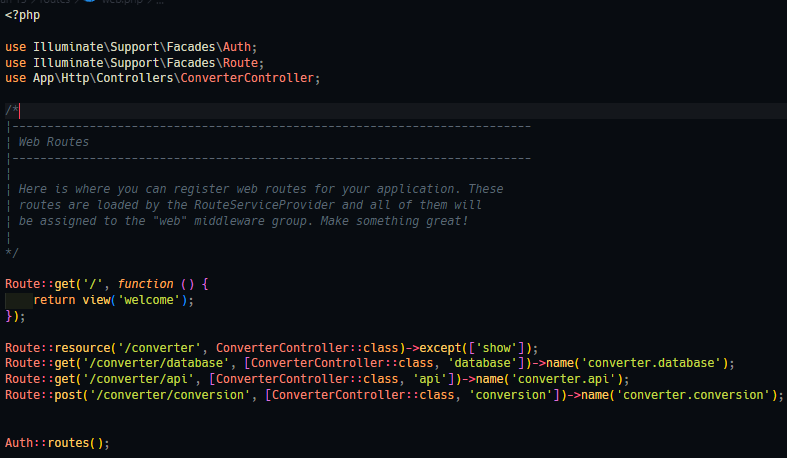
\includegraphics[width=0.6\textwidth]{classFiles/pertemuan-13-converter-routes.png}


        Add conversion function at ConverterController inside Controllers folder
    \end{center}
    \vfill % Pushes content to the bottom of the frame
\end{frame}

\begin{frame}{Add Navigation in app.blade.php}
    \vskip1cm
    \begin{center}
        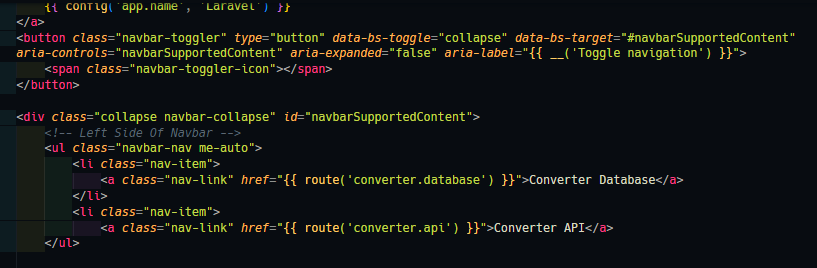
\includegraphics[width=0.6\textwidth]{classFiles/pertemuan-13-app-navigation.png}


        Add Navigation in app.blade.php in folder views/layout
    \end{center}
    \vfill % Pushes content to the bottom of the frame
\end{frame}

\begin{frame4}
    \frametitle{Thank You}
\end{frame4}

\end{document}
